\section{Introduction}\label{sec:intro}

\subsection{Problem restatement}
A smartphone that lasts all day on Monday may be dead by lunch on Tuesday. ``Heavy use'' explains only part of
this. The battery delivers \emph{power} to a load whose size depends on the screen, the processor, the radios and
background software. It does so through an internal resistance that grows in the cold and with age. The phone also
heats itself and throttles itself. We are asked for a \emph{continuous-time} model of the state of charge (SOC)
of a lithium-ion phone battery under realistic use. The model must predict the time-to-empty (TTE) from any
starting charge, explain which activities and conditions drain the battery fastest, quantify uncertainty and
sensitivity, and turn the findings into advice for users and for operating systems (OS).

\subsection{Our approach}
We build a hierarchy of four continuous-time models. Each level adds one physical mechanism, so the effect of
every mechanism on TTE can be measured on its own (\cref{fig:architecture}).
\begin{itemize}
  \item \textbf{L0, energy bucket:} $\dot E=-P(t)$. It gives closed-form TTE and the key insight that each
  component's \emph{energy share} equals the magnitude of its TTE elasticity.
  \item \textbf{L1, quasi-static circuit:} open-circuit voltage $\Ocv(\soc)$ and a series resistance under a
  \emph{constant-power} load. It gives an exact quadrature for TTE and the losses at the cut-off voltage.
  \item \textbf{L2, dynamic electro-thermal circuit (main model):} RC polarization, a lumped thermal node,
  Arrhenius resistance, entropic heat, skin-temperature throttling, and two voltage thresholds: the fuel-gauge
  cut-off under sustained or multi-second loads and a brown-out under sub-second power peaks. Together they
  explain why cold or aged phones die while still showing charge.
  \item \textbf{L3, aging:} slow calendar, solid-electrolyte interphase (SEI) and lithium-plating states. They shrink capacity and raise
  resistance over months.
\end{itemize}
Usage enters as a piecewise-constant input $\bm u(t)$. It is either a deterministic schedule or a continuous-time
Markov chain (CTMC) over activities. The CTMC turns the battery into a piecewise-deterministic Markov process
(PDMP) with closed-form approximations of the mean and variance of TTE. Every parameter is a cited
measurement, an open-data fit or a labeled assumption; one discharge constant is calibrated to phone data and
the two aging rates to the manufacturers' 1000-cycle rating. The model is validated against open-licensed phone
and cell data. \Crefrange{sec:assumptions}{sec:analytic} build the model, \cref{sec:params,sec:validation} fit
and test it, \crefrange{sec:tte}{sec:aging} predict and analyze TTE, and \cref{sec:recs,sec:general} give advice
and generalize; page~2 maps each requirement of the problem to its answer.

\begin{figure}[!b]
  \centering
  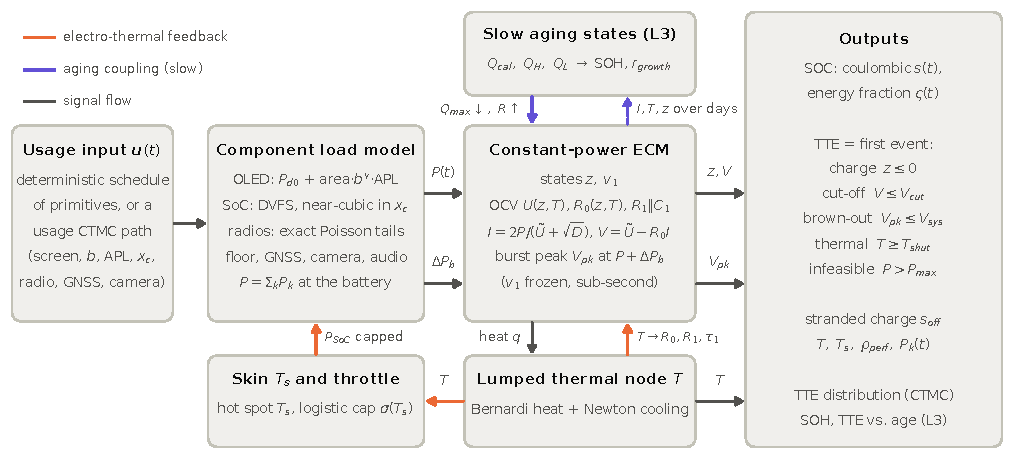
\includegraphics[width=0.92\textwidth]{figures/fig_architecture.pdf}
  \caption{Model architecture. The usage input $\bm u(t)$ drives the component load model. The constant-power
  equivalent-circuit model (ECM) converts power into current, and the thermal node closes two feedback loops:
  temperature sets the resistance, and skin temperature throttles the processor (SoC). Slow aging states (the
  losses $q_{\mathrm{cal}},q_H,q_L$ of \cref{eq:aging}) set capacity and resistance. TTE is the first of five
  events.}
  \label{fig:architecture}
\end{figure}
